\section{Dérivation}

\noindent Nous allons analyser la convection naturelle le long d'une plaque chauffée verticale plane dont le bas se situe en $y=0$.

\begin{itemize}
  \item Le fluide colle à la plaque : $v = 0$ en $x = 0$.
  \item Le fluide est au repos loins de la plaque : $u = v = 0$.
  \item Le fluide est plus chaud proche de la plaque: $T_w > T_e$.
  \item $\delta << Y$
\end{itemize}

\noindent On suppose que l'écoulement n'existe que dans la couche limite ($\delta(x)$). \\
Dès lors on peut utiliser \textbf{les équations de Prandtl} en y ajoutant \textbf{le terme lié à la poussée d'Archimède} et en négligeant \textbf{la dissipation visqueuse}.

\noindent Hypothèses de Prandtl

\begin{itemize}
  \item L'écoulement est à grand nombre de Reynolds.
  \item L'épaisseur de la couche limite dépend du nombre de Reynolds $(\frac{\delta}{Y} = \frac{1}{\sqrt{Re}})$.
  \item Les forces d'inertie, de pression et de viscosité sont du même ordre de grandeur dans la couche limite.
\end{itemize}

\begin{itemize}
  \item Poussée d'Archimède (la pression ne dépend que de la profondeur) : $P(x, y) = \rho g y$
\end{itemize}

\noindent On peut obtenir une solution de similitude en définissant :
\begin{equation}
  \eta(x,y) = \frac{x}{\delta(y)} = \frac{x}{y} \left( \frac{Gr(y)}{4} \right)^{1/4}
\end{equation}

\begin{itemize}
  \item Nombre de Grasshof : $\frac{(\text{"poussée d'Archimède"})(\text{terme d'inertie})}{(\text{forces visqueuses})^2} = \frac{\beta \Delta T g L^3}{\nu^2}$
\end{itemize}

% \definecolor{zzttff}{rgb}{0,0.756,0}
% \begin{figure}[ht!]
%     \centering
% \begin{tikzpicture}
%     \draw[black] (-2,1) -- (2,1);
%     \draw[black, very thick] (0,-4) -- (0,2);
%     \draw[line width=2.pt,color=red,smooth,samples=100,domain=0:1.4] plot(\x,{3*(\x)^(2.0)-4});
%     \draw[zzttff,<->] ( 0,1.05) -- (1.29,1.05);
%     \draw(0.55,1.3) node [zzttff] {$\delta$};
%     \draw[zzttff,<->] (-0.06,-4) -- (-0.06,1) ;
%     \draw(-0.5,-1) node [zzttff] {$L$};
% \end{tikzpicture}
%     \caption{Couche limite}
%     \label{fig:1}
% \end{figure}


\begin{marginfigure}
  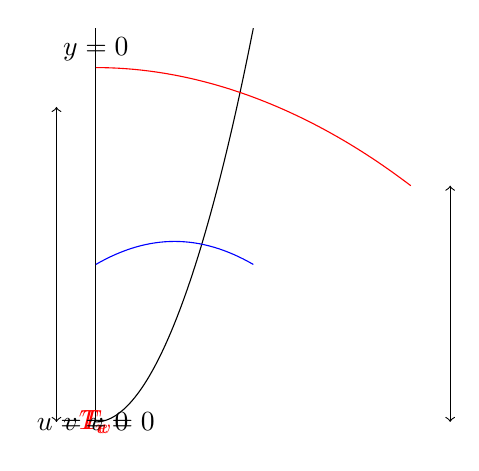
\begin{tikzpicture}
    % plaque chaude
    \draw (0,0) -- (0,5) node [below] {$y=0$};
    % couche limite
    \draw (0,0) parabola (2,5);
    % profil de température
    \node[text=red] (-1,4.5) {$T_w$};
    \draw[red] (0,4.5) parabola (4,3);
    \node[text=red] (2,4) {$T_e$};
    % profil de vitesse
    \node (-1,2) {$v=0$};
    \path (0,2) coordinate (p1);
    \path (2,2) coordinate (p2);
    \draw[blue] (p1) to [bend left] (p2);
    \node (3,4) {$u = v = 0$};
    % axes
    \draw[<->] (-0.5,0) -- (-0.5,4);
    \draw[<->] (4.5,0) -- (4.5,3);
  \end{tikzpicture}
\end{marginfigure}

On part des équations de Navier-Stokes 2D :

\begin{align}
  \pdv{u}{x} + \pdv{v}{y} &= 0 \qq{(\textit{fluide incompressible})} \\
  \rho \left[ u \pdv{u}{x} + v \pdv{u}{y} \right] &= - \pdv{P}{x} + \mu \left[ \pdv[2]{u}{x} + \pdv[2]{u}{y} \right] \qq{(\textit{fluid flow})} \\
  \rho \left[ u \pdv{v}{x} + v \pdv{v}{y} \right] &= - \pdv{P}{y} + \mu \left[ \pdv[2]{v}{x} + \pdv[2]{v}{y} \right] \qq{(\textit{fluid flow})} \\
  u \pdv{T}{x} + v \pdv{T}{y} &= \alpha \left[\pdv[2]{T}{x} + \pdv[2]{T}{y} \right] \qq{(heat flow)}
\end{align}

\newpage

\chapter{\underline{Simplifications :}}

On part du principe que la largeur de la couche limite est beaucoup plus petite que la longueur de la plaque.
Cette simplification va nous permettre de retrouver les équations de Prandtl.

\begin{equation}
  \boxed{\delta << Y}
\end{equation}

On commence par l'équation décrivant l'écoulement incompressible, on peut comparer ses 2 termes d'inerties :

\begin{align*}
  \underbrace{\pdv{u}{x}}_{\mathcal{O}(\frac{U}{\delta})} + \underbrace{\pdv{v}{y}}_{\mathcal{O}(\frac{V}{Y})} = 0
\end{align*}

Par conséquent on trouve un relation importante :

\begin{equation}
  \boxed{U = V \frac{\delta}{Y} << V}
\end{equation}

On continue ensuite avec les 2 équations du bilan de la quantité de mouvement.
\noindent La couche laminaire est le lieu où les \textit{termes d'inerties} sont du même ordre que les \textit{termes visqueux}, on peut donc les comparer.

On prend la première :

\begin{equation*}
  \rho \left[ \underbrace{u \pdv{u}{x}}_{(1)} + \underbrace{v \pdv{u}{y}}_{(2)} \right] = - \pdv{P}{x} + \mu \left[ \underbrace{\pdv[2]{u}{x}}_{(3)} +  \underbrace{\ccancel{\pdv[2]{u}{y}}{red}}_{(4)} \right]
\end{equation*}

\noindent Pour ce qui est des termes d'inertie, le terme $(1)$ est de l'ordre $\frac{U^2}{\delta} = \frac{V^2}{Y^2}\delta$ et le terme $(2)$ est de l'ordre $\frac{VU}{Y} = \frac{V^2}{Y^2}\delta$ \\
\noindent Pour ce qui est des termes visqueux, le terme $(3)$ est de l'ordre $\frac{U}{\delta^2}$ et le terme $(4)$ est de l'ordre $\frac{U}{Y^2}$.

On observe donc que :

\begin{equation*}
  \boxed{\frac{U}{\delta^2} >> \frac{U}{Y^2} \qq{\textit{le terme $(4)$ est négligeable}}}
\end{equation*}

On peut effectuer un raisonnement similaire avec la seconde équation :

\begin{equation*}
  \rho \left[ \underbrace{u \pdv{v}{x}}_{(1)} + \underbrace{v \pdv{v}{y}}_{(2)} \right] = - \pdv{P}{y} + \mu \left[ \underbrace{\pdv[2]{v}{x}}_{(3)} + \underbrace{\ccancel{\pdv[2]{v}{y}}{red}}_{(4)} \right]
\end{equation*}

% Comparer les termes d'inerties et visqueux. Mettre les ordres "inline" dans le texte ne semble pas très joli.
\noindent Les termes d'inerties sont de l'ordre :

\begin{equation*}
  \systeme{
    u \pdv{v}{x} \approx \mathcal{O}(\frac{UV}{\delta}) = \mathcal{O}(\frac{V^2}{Y}),
    v \pdv{u}{y} \approx \mathcal{O}(\frac{V^2}{Y})
  }
\end{equation*}

\noindent Les termes visqueux sont de l'ordre :

\begin{equation*}
  \systeme{
    \pdv[2]{v}{x} \approx \mathcal{O}(\frac{V}{\delta^2}),
    \pdv[2]{v}{y} \approx \mathcal{O}(\frac{V}{Y^2})
  }
  \implies \frac{V}{\delta^2} >> \frac{V}{Y^2}
\end{equation*}

On peut trouver une autre condition importante à la validité des équations de Prandtl. \\
\noindent Puisque les \textit{termes d'inerties} sont du même ordre que les \textit{termes visqueux}, on peut écrire :

\begin{equation*}
  \rho \frac{V^2}{Y} = \mu \frac{V}{\delta^2} \implies \frac{\delta^2}{Y^2} = \frac{\mu}{V \rho Y} = \frac{1}{Re_y}
\end{equation*}

On trouve donc que l'hypothèse $\delta << Y$ est satisfaite pour un grand nombre de Reynolds :

\begin{equation}
  \boxed{\frac{\delta}{Y} = \frac{1}{\sqrt{Re_y}}}
\end{equation}

Pour ce qui est de la pression, on peut faire un développement de Taylor afin de connaitre la pression dans la zone de la couche laminaire.


Pression dans la couche laminaire $x \sim \mathcal{O}(\delta)$ :

\begin{equation*}
  \boxed{P(x,y) - P_0 \approx P(\delta, y) - P_0 + \ccancel{\pdv{P(x,y)}{x} \biggr\rvert_{x=0} (x - \delta)}{red} + ...}
\end{equation*}

On observe que :

\begin{equation*}
  P(\delta, y) - P_0 = y \pdv{P}{y} \approx \mathcal{O}(Y) \mathcal{O}(\frac{\rho V^2}{Y}) = \mathcal{O}(\rho V^2)
\end{equation*}

\begin{equation*}
  \pdv{P(x,y)}{x} (x - \delta) \approx \mathcal{O}(\frac{\rho U V}{Y}) \mathcal{O}(\delta) = \mathcal{O}(\rho V^2 \frac{\delta^2}{Y^2})
\end{equation*}

\noindent Par conséquent, la pression est constante sur une tranche \underline{horizontale} : $P(y)$ \\
\noindent $\pdv{P}{x}$ étant négligeable, on peut supprimer l'équation contenant ce terme.


\underline{On obtient les équations de Prandtl} :

\begin{align*}
  %\boxed{
    \pdv{u}{x} + \pdv{v}{y} &= 0 \\
    \left[ u \pdv{v}{x} + v \pdv{v}{y} \right] &= - \frac{1}{\rho} \dv{P}{y} + \nu \left[ \pdv[2]{v}{x} \right]
  %}
\end{align*}


